% Mirror: https://github.com/SIGma-UIUC/presentation-format
% --------------------------------------------------------------------
% This is a simple Beamer document that uses beamerthemesigma.sty
% Reading the comments should help you create a presentation even if
% you've never used Beamer before.
% --------------------------------------------------------------------

% Set our document class to Beamer
\documentclass[aspectratio=169]{beamer}
% \documentclass[aspectratio=169, handout]{beamer}
% Add handout option to ignore pauses

% From Jeff E
\usepackage{algo}
% Some more macros
\usepackage{sigmastyle}


% Set a title
\title{Convex Hulls}

% Set a subtitle if you desire
\subtitle{Adapted from CS498TC \cite{site:jeff}}

% Whoever worked on the presentation:
\author{Sam Ruggerio}

% Date looks ugly, so leave blank
\date{}

% An institute name, if you're so inclined
% \institute{University of Illinois Urbana-Champaign}

% Use the SIGma theme for this Beamer presentation
\usetheme{sigma}
% --------------------------------------------------------------------

% Begin document
\begin{document}

% Beamer calls each slide a "frame", defined within the environment:
% \begin{frame}
%   <frame content here>
% \end{frame}

% This frame is just the title.
\begin{frame}
\titlepage
\end{frame}

% A frame with the table of contents.
% This frame's title is "Outline".
\begin{frame}{Outline}
  \tableofcontents
\end{frame}

% \begin{frame}{Updates!}
%   % Let's put some real content in this frame:
%   Weekly updates:
%   \begin{itemize}
%     \item SIGma is an excellent SIG.
%     \item I'm out of ideas for updates.
%   \end{itemize}
% \end{frame}

% Start a section: *sections* (subsections, etc.) are what show up in the TOC.
\section{Computational Geometry}
\frame{\sectionpage}

\begin{frame}{What is Computational Geometry}
    \begin{itemize}
        \item Algorithms and data structures with discrete geometric objects! \pause 
        \item Working with points, lines, polygons, planes, polytopes, etc. \pause
        \item Low dimensional computational geometry has applications in graphics, motion planning, modeling, mesh processing, etc. \pause 
        \item High dimensional CG is the basis of many ML algorithms. \pause 
        \item (The part of theory with cool pictures)
    \end{itemize}
\end{frame}

\begin{frame}{Assumptions}
    \begin{itemize}
        \item We will often deal with items in real space ($\mathbb{R}^d$)
        \item This means having to do math with real numbers (including roots if we ever want to find distances) \pause
        \item So our model of computation is the \textbf{Real RAM}: \pause
        \begin{itemize}
            \item $+,-,/,\times, \sqrt{x}, x=0?, x>0?$ are all $O(1)$ time between real numbers
            \item Each number takes $O(1)$ space (no bit complexity)
            \item Stored exactly (no floating point)
            \item Notably, transcendental functions are not supported (e.g. $sin, cos, tan$).
        \end{itemize}
    \end{itemize}
\end{frame}

\begin{frame}{Assumptions}
    \begin{itemize}
        \item Points placed in the plane can construct many other objects (circles, lines, etc...) \pause
        \item Often, we want to refer to these structures (relatively) uniquely, without degenerate cases. \pause
        \item Our assumption for most problems will be \textbf{General Position:} \pause
        \begin{itemize}
            \item No two points are in the same position
            \item No three points are co-linear
            \item No four points are co-circular \pause
        \end{itemize}
        \item General position is a simplification, you can (almost) always change an input set to general position, or design an algorithm to handle special position.
    \end{itemize}
\end{frame}

\begin{frame}{Definitions}
    \begin{itemize}
        \item A Polygon $Q$ is an \textit{ordered} circular sequence of Points $P$.
        \item A polygon is \textit{simple} if it does not self-intersect or have holes
        \item A polygon is \textit{convex} if $\forall p,q \in Q, \overline{pq} \in Q$.
        \item A polygon is \textit{closed} if there is a segment for each pair of adjacent points in $P$.
    \end{itemize}
\end{frame}

\begin{frame}{Polygons}
\begin{center}
        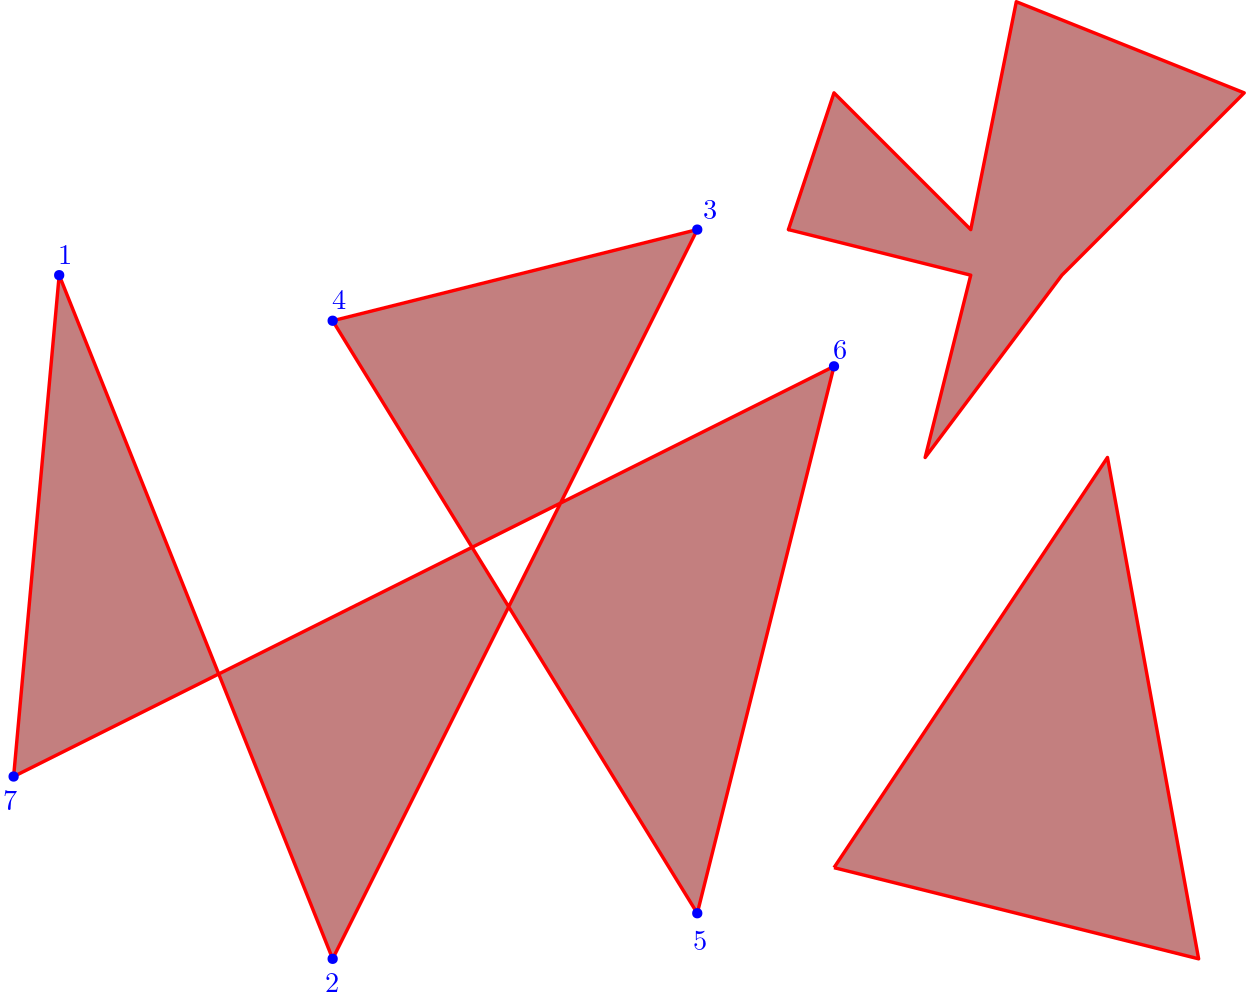
\includegraphics[width=.75\textwidth]{polys.png}
\end{center}
\end{frame}

\section{Convex Hulls}
\frame{\sectionpage}

\begin{frame}{Convex Hulls}
    \begin{itemize}
        \item Problem: Given a point set $P$, we want to compute the \textit{convex hull} $Q$ 
    \end{itemize}
    \begin{center}
    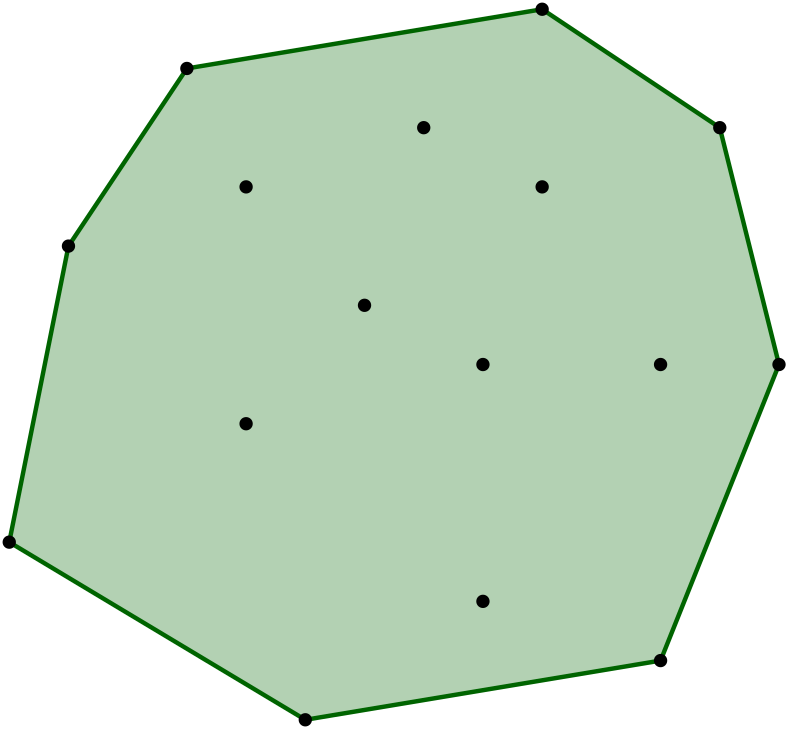
\includegraphics[width = .5\textwidth]{convexhull.png}    
    \end{center}
\end{frame}

\begin{frame}{Convex Hulls}
    \begin{itemize}
        \item Intuitively, we want to place a rubber band around all the points. \pause
        \item Formally, we want to compute the smallest convex polygon containing all the points. \pause
        \item We can describe an algorithm which just \textit{wraps} the polygon.
    \end{itemize}
\end{frame}

\begin{frame}{Jarvis March}
Jarvis March algorithm computes a convex hull via the following:
    \begin{itemize}
        \item Find the leftmost point $\ell$, set as current point. \pause
        \item Repeat until we return to $\ell$: \pause 
        \begin{itemize}
            \item Compare slope of each point relative to current point \pause 
            \item Pick point with least slope, add to hull and set as current point. \pause
        \end{itemize}
        \item We could go clockwise and pick greatest slope, by convention polygons are given in counter-clockwise order.
    \end{itemize}
\end{frame}

\begin{frame}{Jarvis March}
    \begin{center}
        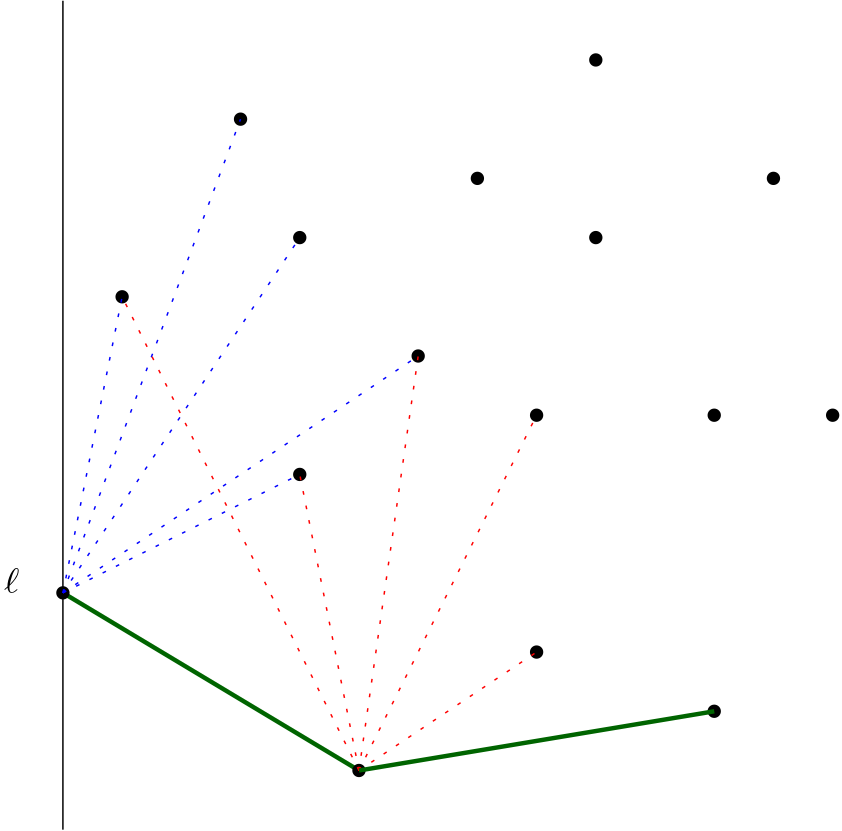
\includegraphics[width=.60\textwidth]{jarvis.png}
    \end{center}
\end{frame}

\begin{frame}{Jarvis March}
    Runtime? \pause
    \begin{itemize}
        \item $O(n)$ to find leftmost point \pause
        \item $O(n)$ slopes to compare \pause 
        \item Repeat for each point on the hull, $h$, $O(h)$ times. \pause
        \item $O(nh) \implies O(n^2)$ in the worst case.
    \end{itemize}
    Jarvis March is \textit{output sensitive}. It does better when the output structure is small.
\end{frame}

\begin{frame}{Doing Better}
    \begin{itemize}
        \item Jarvis March is the slightly-clever version of a brute force solution. \pause
        \item But convex hulls are nice structures! Surely we can exploit some property \pause
        \item We might be able to provide a greedy solution based off of local convexity \pause
        \item If a 2D simple polygon is locally convex everywhere, it must be convex. \pause
        \item But how do we test convexity?
    \end{itemize}
\end{frame}

\begin{frame}{Orientation}
\begin{itemize}
    \item We have a circular sequence of points, which means the ordering of points can be viewed as \textit{clockwise} or \textit{counter-clockwise}
\end{itemize}
\begin{center}
    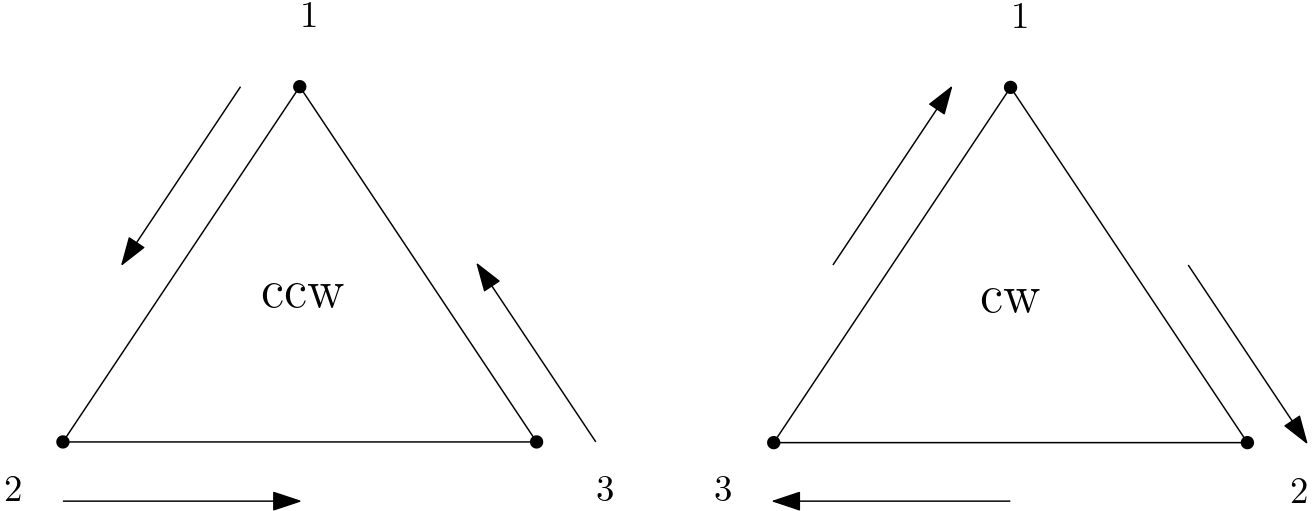
\includegraphics[width=.5\textwidth]{orientation.png}
\end{center}
\begin{itemize}
    \item We determine orientation based off of the slope between one point and the rest.
\end{itemize}
\end{frame}

\begin{frame}{Orientation Test}
    \begin{itemize}
        \item Assume $p_1$ is the leftmost point of $p_1,p_2,p_3$, then:
        \begin{itemize}
            \item If the slope $\overline{p_1p_2}$ is greater than $\overline{p_1p_3}$, it's clockwise
            \item Otherwise, it's counterclockwise \pause 
            \item (If it's equal, its flat, which shouldn't happen under general position)
        \end{itemize}
        \item To simplify, we're doing the following test: $$\frac{y_2-y_1}{x_2-x_1} > \frac{y_3 - y_1}{x_3-x_1}$$
    \end{itemize}
\end{frame}

\begin{frame}{It's just math!}
    Following through:
    \begin{align*}
        \frac{y_2-y_1}{x_2-x_1} &> \frac{y_3 - y_1}{x_3-x_1} \\
        y_2x_3-y_2x_1-y_1x_3+y_1x_1 &> y_3x_2 - y_1x_2 - y_3x_1 + y_1x_1 \\
        y_1x_2+y_3x_1-y_3x_2+y_2x_3-y_2x_1-y_1x_3 &> 0
    \end{align*}
\end{frame}

\begin{frame}{It's just math!}
    Following through:
    \begin{align*}
        \frac{y_2-y_1}{x_2-x_1} &> \frac{y_3 - y_1}{x_3-x_1} \\
        y_2x_3-y_2x_1-y_1x_3+y_1x_1 &> y_3x_2 - y_1x_2 - y_3x_1 + y_1x_1 \\
        y_1x_2+y_3x_1-y_3x_2+y_2x_3-y_2x_1-y_1x_3 &> 0 \\ 
        \begin{vmatrix}
     1 & x_1 & y_1\\ 
     1 & x_2 & y_2\\
     1 & x_3 & y_3 
     \end{vmatrix} &> 0
    \end{align*}
    Recall that the determinant of 3 points in that form gives you 2 times the area of a triangle. Positive if it's ccw, negative if cw.
\end{frame}

\begin{frame}{Orientation Test}
    \begin{itemize}
        \item Take the (signed) determinant of 3 points
        \item If greater than 0, points are oriented counter clockwise
        \item If less than 0, points are oriented clockwise
        \item If equal to 0, points are flat. \pause
        \item Runtime? \pause $O(1)$
    \end{itemize}
\end{frame}

\begin{frame}{Graham's Scan}
    \begin{itemize}
        \item First, find the leftmost point $\ell$
        \item Then, create a polygon $Q$, sorted around $\ell$
    \end{itemize}
    \begin{center}
        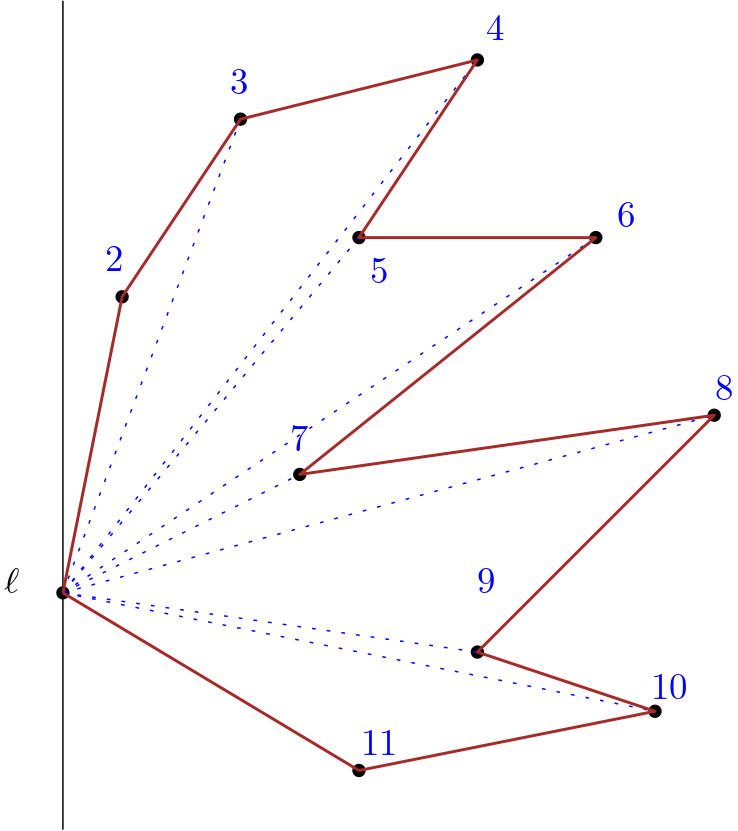
\includegraphics[width=.4\textwidth]{graham_pt1.png}
    \end{center}
\end{frame}

\begin{frame}{Graham's Scan}
    \begin{itemize}
        \item Then, perform a repair on the polygon:
        \begin{itemize}
            \item Mark the first 3 vertices \pause
            \item If they are convex, move all marks forward one vertex \pause
            \item If not, delete the middle mark, and mark the previous vertex \pause
            \item Repeat.
        \end{itemize}
    \end{itemize}
\end{frame}

\begin{frame}{Graham's Scan}
    \begin{center}
        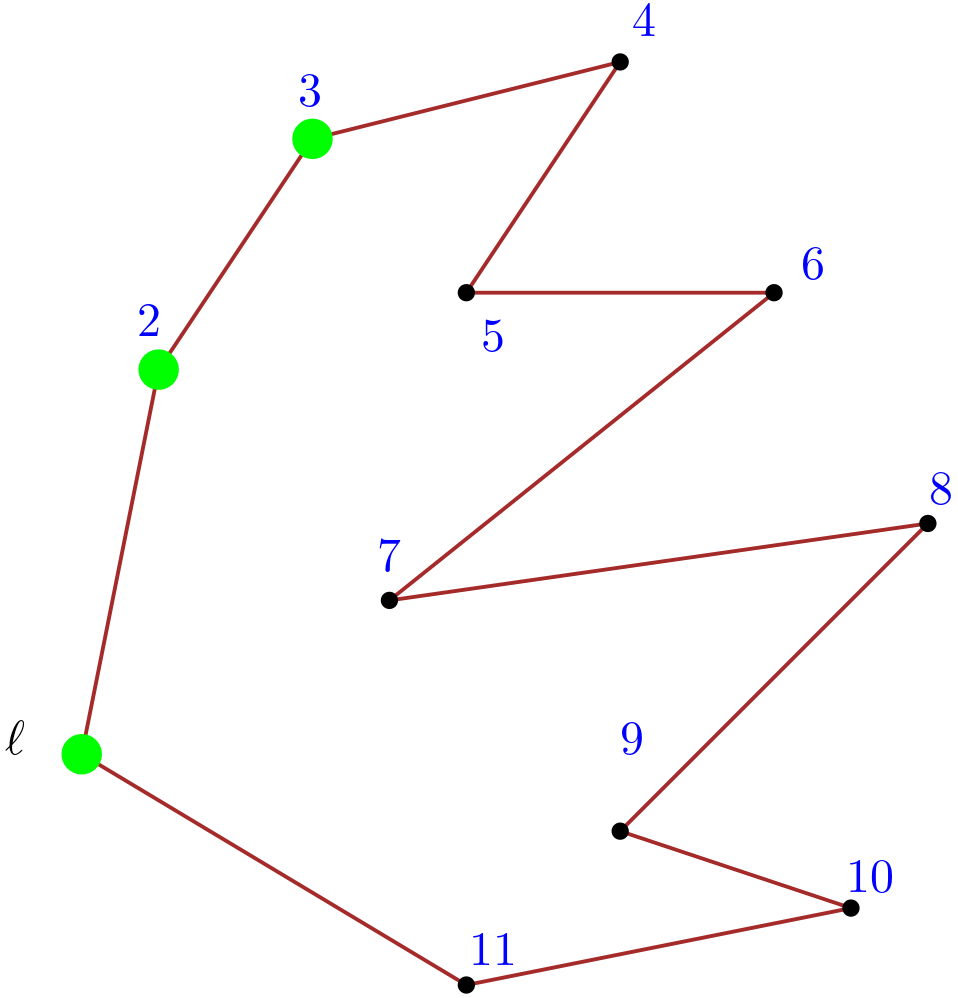
\includegraphics[width=.5\textwidth]{graham_pt2.png}
    \end{center}
\end{frame}

\begin{frame}{Graham's Scan}
    \begin{center}
        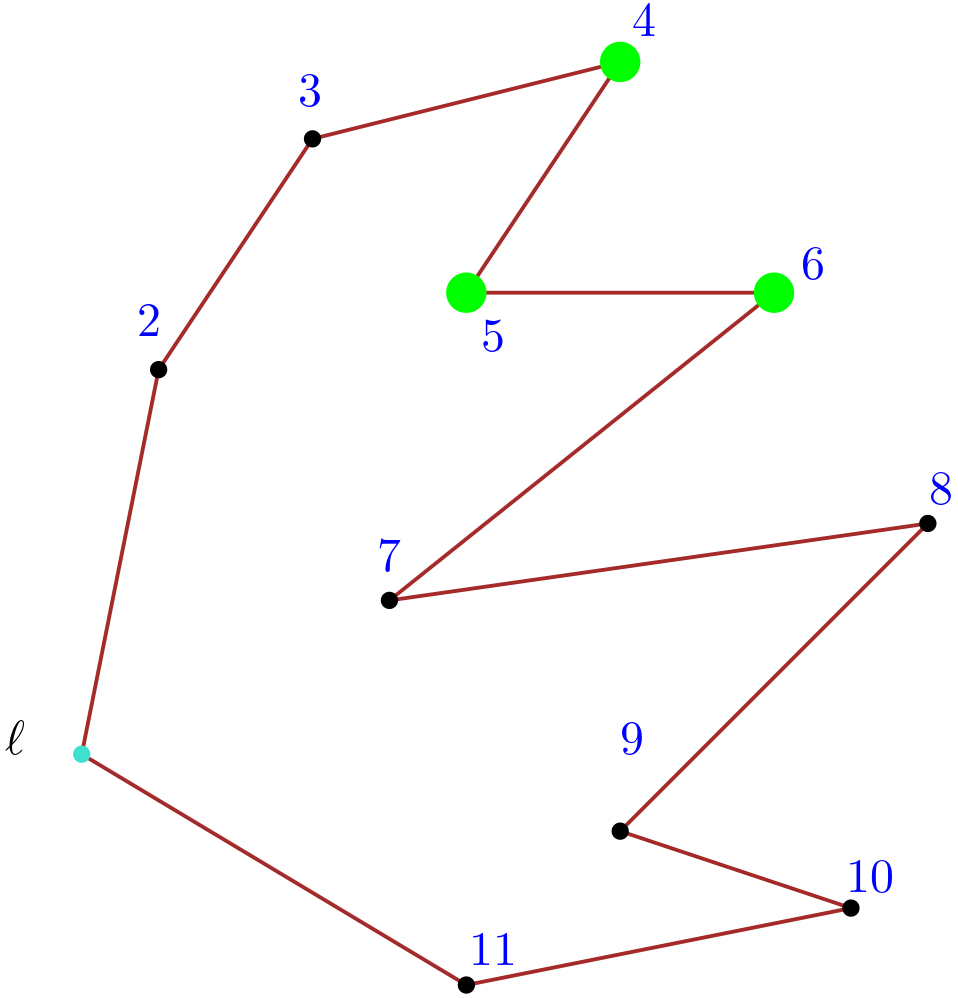
\includegraphics[width=.5\textwidth]{graham_pt3.png}
    \end{center}
\end{frame}

\begin{frame}{Graham's Scan}
    \begin{center}
        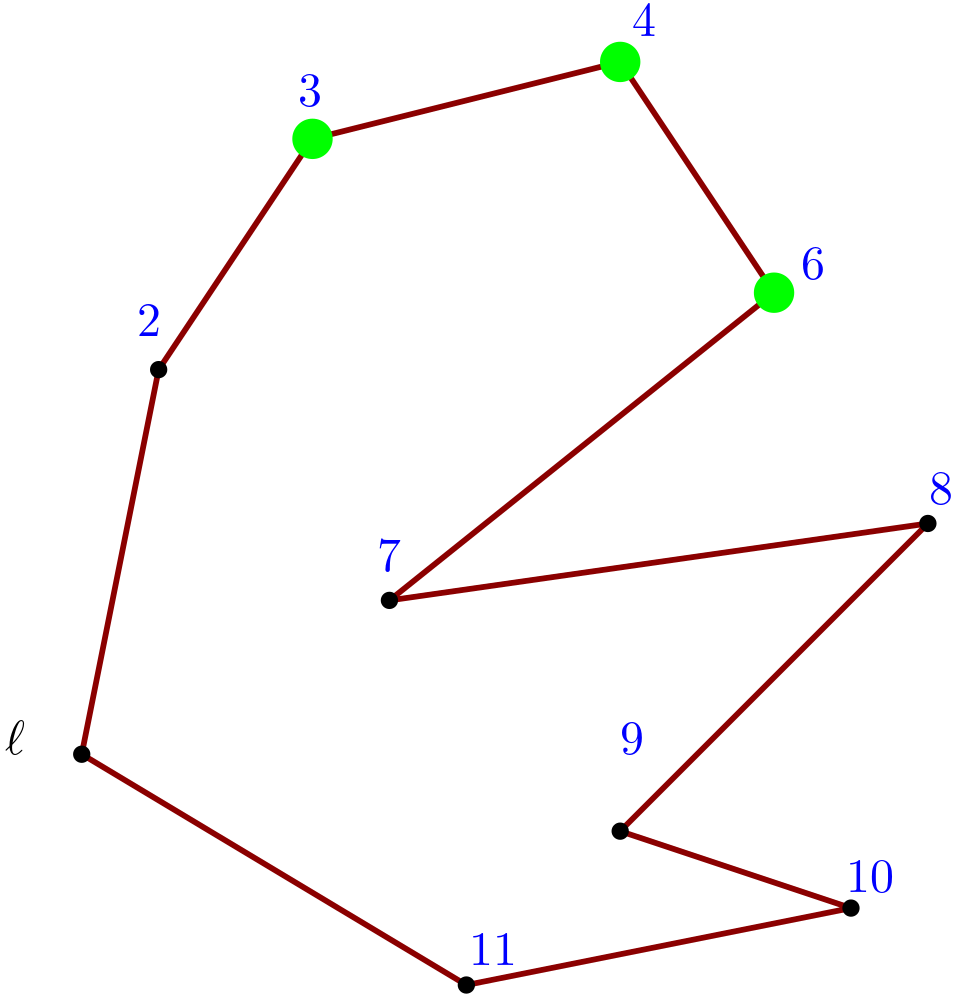
\includegraphics[width=.5\textwidth]{graham_pt4.png}
    \end{center}
\end{frame}

\begin{frame}{Graham's Scan}
    Runtime?
    \begin{itemize}
        \item Find leftmost point: $O(n)$ \pause 
        \item Sort points around $\ell$ to construct a polygon: $O(n \log n)$ \pause
        \item 3 mark repair? \pause
        \begin{itemize}
            \item You could delete at most $O(n)$ points \pause
            \item Each deletion moves the marks back one spot \pause
            \item Otherwise, the scan moves forward one spot $\implies O(n)$ time. \pause
        \end{itemize}
        \item $O(n \log n)$ total runtime (dominated by sort)
    \end{itemize}
\end{frame}


\section{Optimal Convex Hulls}
\frame{\sectionpage}

\begin{frame}{Doing Even Better}
    \begin{itemize}
    \item We have an output sensitive but slow algorithm in $O(nh)$
    \item We have a fast, sorting-bound algorithm in $O(n \log n)$
    \item Can we get a fast output sensitive algorithm?
    \end{itemize}
\end{frame}

\begin{frame}{Chan's Algorithm}
\begin{itemize}
    \item In 1996, Timothy Chan (UIUC) came up with an output-sensitive \textit{optimal} 2D convex hull algorithm \pause
    \item We'll use both Jarvis March and Graham's Scan within our process.
    \item The high level idea is to construct a cluster of small convex hulls and merge them
\end{itemize}
\end{frame}

\begin{frame}{Shattering the Hulls}
    \begin{itemize}
        \item Let $h$ be a number we'll determine later. \pause
        \item Break our input set $P$ into $O(n/h)$ subsets of size $O(h)$. \pause 
        \item Compute the convex hull of each subset using Graham's Scan: \pause 
        \begin{itemize}
            \item $O(n/h)$ subsets, each of size $O(h)$, thus taking $h \log h$ time, in total $n \log h$ time.
        \end{itemize}
    \end{itemize}
\end{frame}

\begin{frame}{Candidate Points}
    \begin{itemize}
        \item We need to pick final output vertices
        \item In each hull, we need a candidate point, we pick the lowest tangent point relative to our current output vertex.
        \item We'll find this candidate point via binary search on the hull.
    \end{itemize}
\end{frame}

\begin{frame}{Binary Search on Hulls}
    \begin{itemize}
        \item We want to find the lower tangent of a hull $H$ from some start point $\ell$
    \end{itemize}
    \begin{center}
        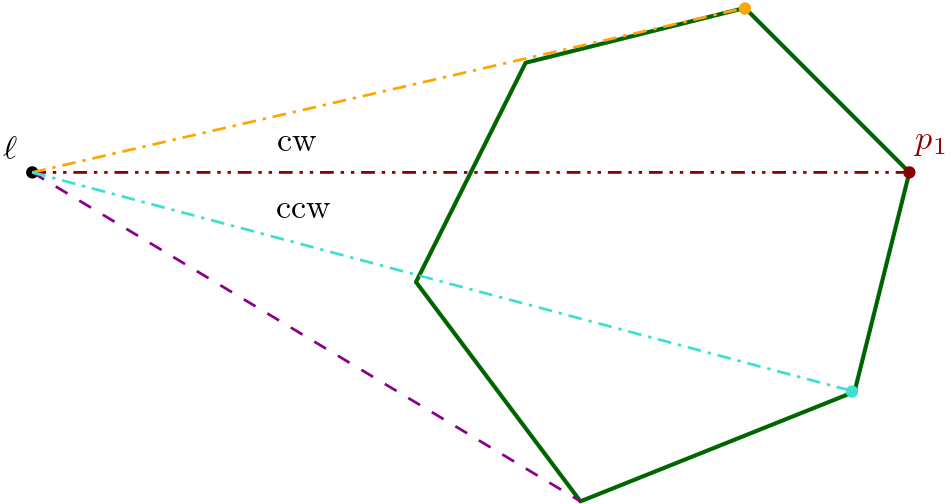
\includegraphics[width=.6\textwidth]{binsearch.png}
    \end{center} \pause
    \begin{itemize}
        \item Once the orientation changes from cw, ccw, we found our point.
    \end{itemize}
\end{frame}

\begin{frame}{Putting It Together}
    \begin{itemize}
        \item We can now select candidate points from our sub-hulls and create a global convex hull:
    \end{itemize}
    \begin{center}
        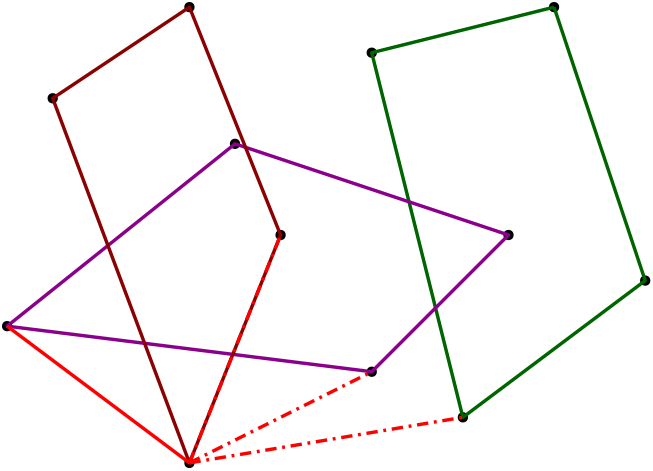
\includegraphics[width=.6\textwidth]{hull-select.png}
    \end{center}
\end{frame}

\begin{frame}{Runtime}
    \begin{itemize}
        \item For each output vertex, in total $h$ times: \pause
        \begin{itemize}
            \item We find our next candidate point via binary search in each subset
            \item $O(n/h) \times O( \log h)$
            \item Total: $O(n \log h)$ \pause
        \end{itemize}
        \item Combined with our Graham's scan, we get a final runtime of $O(n \log h)$ \pause
        \item How do we determine the number of output points ahead of time??
    \end{itemize}
\end{frame}

\begin{frame}{Exponential Search}
    \begin{itemize}
        \item Search $h$ via exponential search, $h=3, 9, 81, \dots, 3^{2^k} = h_k$ \pause 
        \item If you don't output a hull with the number of vertices guessed, you try again! \pause
        \item $O(n \log h_1 + n \log h_2 + n \log h_3 + \cdots n \log h^2)$ \pause
        \begin{itemize}
            \item This exponential doubling will eventually exceed $h$, but no more than $h^2$ \pause
        \end{itemize}
        \item $O(n \log 3 + 2 n \log 3 + \dots 2^k n \log 3) \leq O(n \log h^2) \implies O(n \log h)$
    \end{itemize}
\end{frame}

\begin{frame}{Other things to think about!}
    \begin{itemize}
        \item Convex Hulls in 3D? in n-D?
        \item Triangulating polygons?
        \item Test if a point is inside a non-simple polygon?
        \item Linear Programming from a CG perspective
        \item Shortest Paths in 2D space, or in planar graphs?
    \end{itemize}
\end{frame}

\begin{frame}{}
      \begin{center}
    {\color{sigma@mainblue} \LARGE Questions?}
  \end{center}
\end{frame}

% Remove this slide if you came up with all the material yourself
\begin{frame}[allowframebreaks]{Bibliography}
    \tiny
    \bibliography{refs}
    \bibliographystyle{alpha}
\end{frame}

\end{document}